% Options for packages loaded elsewhere
\PassOptionsToPackage{unicode}{hyperref}
\PassOptionsToPackage{hyphens}{url}
%
\documentclass[
]{article}
\usepackage{amsmath,amssymb}
\usepackage{lmodern}
\usepackage{ifxetex,ifluatex}
\ifnum 0\ifxetex 1\fi\ifluatex 1\fi=0 % if pdftex
  \usepackage[T1]{fontenc}
  \usepackage[utf8]{inputenc}
  \usepackage{textcomp} % provide euro and other symbols
\else % if luatex or xetex
  \usepackage{unicode-math}
  \defaultfontfeatures{Scale=MatchLowercase}
  \defaultfontfeatures[\rmfamily]{Ligatures=TeX,Scale=1}
\fi
% Use upquote if available, for straight quotes in verbatim environments
\IfFileExists{upquote.sty}{\usepackage{upquote}}{}
\IfFileExists{microtype.sty}{% use microtype if available
  \usepackage[]{microtype}
  \UseMicrotypeSet[protrusion]{basicmath} % disable protrusion for tt fonts
}{}
\makeatletter
\@ifundefined{KOMAClassName}{% if non-KOMA class
  \IfFileExists{parskip.sty}{%
    \usepackage{parskip}
  }{% else
    \setlength{\parindent}{0pt}
    \setlength{\parskip}{6pt plus 2pt minus 1pt}}
}{% if KOMA class
  \KOMAoptions{parskip=half}}
\makeatother
\usepackage{xcolor}
\IfFileExists{xurl.sty}{\usepackage{xurl}}{} % add URL line breaks if available
\IfFileExists{bookmark.sty}{\usepackage{bookmark}}{\usepackage{hyperref}}
\hypersetup{
  pdftitle={Linear modeling - R basics},
  pdfauthor={Franz Mueter, with thanks to Arni Magnusson},
  hidelinks,
  pdfcreator={LaTeX via pandoc}}
\urlstyle{same} % disable monospaced font for URLs
\usepackage[margin=1in]{geometry}
\usepackage{color}
\usepackage{fancyvrb}
\newcommand{\VerbBar}{|}
\newcommand{\VERB}{\Verb[commandchars=\\\{\}]}
\DefineVerbatimEnvironment{Highlighting}{Verbatim}{commandchars=\\\{\}}
% Add ',fontsize=\small' for more characters per line
\usepackage{framed}
\definecolor{shadecolor}{RGB}{248,248,248}
\newenvironment{Shaded}{\begin{snugshade}}{\end{snugshade}}
\newcommand{\AlertTok}[1]{\textcolor[rgb]{0.94,0.16,0.16}{#1}}
\newcommand{\AnnotationTok}[1]{\textcolor[rgb]{0.56,0.35,0.01}{\textbf{\textit{#1}}}}
\newcommand{\AttributeTok}[1]{\textcolor[rgb]{0.77,0.63,0.00}{#1}}
\newcommand{\BaseNTok}[1]{\textcolor[rgb]{0.00,0.00,0.81}{#1}}
\newcommand{\BuiltInTok}[1]{#1}
\newcommand{\CharTok}[1]{\textcolor[rgb]{0.31,0.60,0.02}{#1}}
\newcommand{\CommentTok}[1]{\textcolor[rgb]{0.56,0.35,0.01}{\textit{#1}}}
\newcommand{\CommentVarTok}[1]{\textcolor[rgb]{0.56,0.35,0.01}{\textbf{\textit{#1}}}}
\newcommand{\ConstantTok}[1]{\textcolor[rgb]{0.00,0.00,0.00}{#1}}
\newcommand{\ControlFlowTok}[1]{\textcolor[rgb]{0.13,0.29,0.53}{\textbf{#1}}}
\newcommand{\DataTypeTok}[1]{\textcolor[rgb]{0.13,0.29,0.53}{#1}}
\newcommand{\DecValTok}[1]{\textcolor[rgb]{0.00,0.00,0.81}{#1}}
\newcommand{\DocumentationTok}[1]{\textcolor[rgb]{0.56,0.35,0.01}{\textbf{\textit{#1}}}}
\newcommand{\ErrorTok}[1]{\textcolor[rgb]{0.64,0.00,0.00}{\textbf{#1}}}
\newcommand{\ExtensionTok}[1]{#1}
\newcommand{\FloatTok}[1]{\textcolor[rgb]{0.00,0.00,0.81}{#1}}
\newcommand{\FunctionTok}[1]{\textcolor[rgb]{0.00,0.00,0.00}{#1}}
\newcommand{\ImportTok}[1]{#1}
\newcommand{\InformationTok}[1]{\textcolor[rgb]{0.56,0.35,0.01}{\textbf{\textit{#1}}}}
\newcommand{\KeywordTok}[1]{\textcolor[rgb]{0.13,0.29,0.53}{\textbf{#1}}}
\newcommand{\NormalTok}[1]{#1}
\newcommand{\OperatorTok}[1]{\textcolor[rgb]{0.81,0.36,0.00}{\textbf{#1}}}
\newcommand{\OtherTok}[1]{\textcolor[rgb]{0.56,0.35,0.01}{#1}}
\newcommand{\PreprocessorTok}[1]{\textcolor[rgb]{0.56,0.35,0.01}{\textit{#1}}}
\newcommand{\RegionMarkerTok}[1]{#1}
\newcommand{\SpecialCharTok}[1]{\textcolor[rgb]{0.00,0.00,0.00}{#1}}
\newcommand{\SpecialStringTok}[1]{\textcolor[rgb]{0.31,0.60,0.02}{#1}}
\newcommand{\StringTok}[1]{\textcolor[rgb]{0.31,0.60,0.02}{#1}}
\newcommand{\VariableTok}[1]{\textcolor[rgb]{0.00,0.00,0.00}{#1}}
\newcommand{\VerbatimStringTok}[1]{\textcolor[rgb]{0.31,0.60,0.02}{#1}}
\newcommand{\WarningTok}[1]{\textcolor[rgb]{0.56,0.35,0.01}{\textbf{\textit{#1}}}}
\usepackage{graphicx}
\makeatletter
\def\maxwidth{\ifdim\Gin@nat@width>\linewidth\linewidth\else\Gin@nat@width\fi}
\def\maxheight{\ifdim\Gin@nat@height>\textheight\textheight\else\Gin@nat@height\fi}
\makeatother
% Scale images if necessary, so that they will not overflow the page
% margins by default, and it is still possible to overwrite the defaults
% using explicit options in \includegraphics[width, height, ...]{}
\setkeys{Gin}{width=\maxwidth,height=\maxheight,keepaspectratio}
% Set default figure placement to htbp
\makeatletter
\def\fps@figure{htbp}
\makeatother
\setlength{\emergencystretch}{3em} % prevent overfull lines
\providecommand{\tightlist}{%
  \setlength{\itemsep}{0pt}\setlength{\parskip}{0pt}}
\setcounter{secnumdepth}{-\maxdimen} % remove section numbering
\ifluatex
  \usepackage{selnolig}  % disable illegal ligatures
\fi

\title{Linear modeling - R basics}
\author{Franz Mueter, with thanks to Arni Magnusson}
\date{September 7, 2021}

\begin{document}
\maketitle

(Approximate duration: 3 hours)

\hypertarget{model-formulas}{%
\section{Model formulas:}\label{model-formulas}}

There are many uses for formulas in both model fitting functions and in
many graphics functions. Here, we are primarily concerned with formulae
used in modeling functions such as lm, aov, glm, gls, nls, etc. These
functions take a formula as their first argument, which has the general
form:

\texttt{response\ \textasciitilde{}\ expression}

where `response' typically is a response variable or some expression
that returns the response variable, e.g.~\texttt{log(y+1)}, and
`expression' consists of one or more terms (typically the independent
variables in a regression) joined by operators like `+', `-', '*', etc.
In linear and generalized linear modeling the formula specifies how the
response is modeled as a function of the independent variables.

See module 9 slides for more on model formulas and formula notation.

\hypertarget{statistical-modelling-in-r}{%
\section{Statistical modelling in R}\label{statistical-modelling-in-r}}

Let's start by looking at a fairly simple data set to do some basic
model explorations. This is where that regression class comes in handy
that is technically a requirement of the class (!). If you need to brush
up on your regression skills, I suggest Chapter 9 of Gotelli and Ellison
(2004). I posted a pdf on Blackboard.

First, just run through the example code below if you opened the R
Markdown file or by running the script file `Module 9.R'. (Or enter code
in the console, if you prefer)

Look at the mammal data set, which contains brain and body weights for a
number of mammal species:

\begin{Shaded}
\begin{Highlighting}[]
\FunctionTok{library}\NormalTok{(MASS)           }\CommentTok{\# attach MASS library for data and functions}
\NormalTok{mammals           }\CommentTok{\# Look at the mammal data}
\end{Highlighting}
\end{Shaded}

First, as always, explore data graphically, in this case there aren't a
whole lot of clever things to do except looking at a simple scatterplot.
It makes sense that brain size may be related to and determined by body
size (rather than the other way around), hence we plot body size on the
x-axis and use it as the `explanatory' variable in modeling.

\begin{Shaded}
\begin{Highlighting}[]
\FunctionTok{plot}\NormalTok{(brain }\SpecialCharTok{\textasciitilde{}}\NormalTok{ body, }\AttributeTok{data=}\NormalTok{mammals)}
\end{Highlighting}
\end{Shaded}

\includegraphics{Lab-5-Linear-Models_files/figure-latex/unnamed-chunk-1-1.pdf}

Note the curvature in the relationship and the fact that there are a
couple awfully big animals that make everyone else appear tiny (Who are
they? You could look at the sorted data frame to find out). Both of
those observations suggest that a log-transformation may be appropriate
(although that may not be obvious to you at this point).

Let's try it:

\begin{Shaded}
\begin{Highlighting}[]
\FunctionTok{plot}\NormalTok{(}\FunctionTok{log}\NormalTok{(brain) }\SpecialCharTok{\textasciitilde{}} \FunctionTok{log}\NormalTok{(body), }\AttributeTok{data=}\NormalTok{mammals)}
\end{Highlighting}
\end{Shaded}

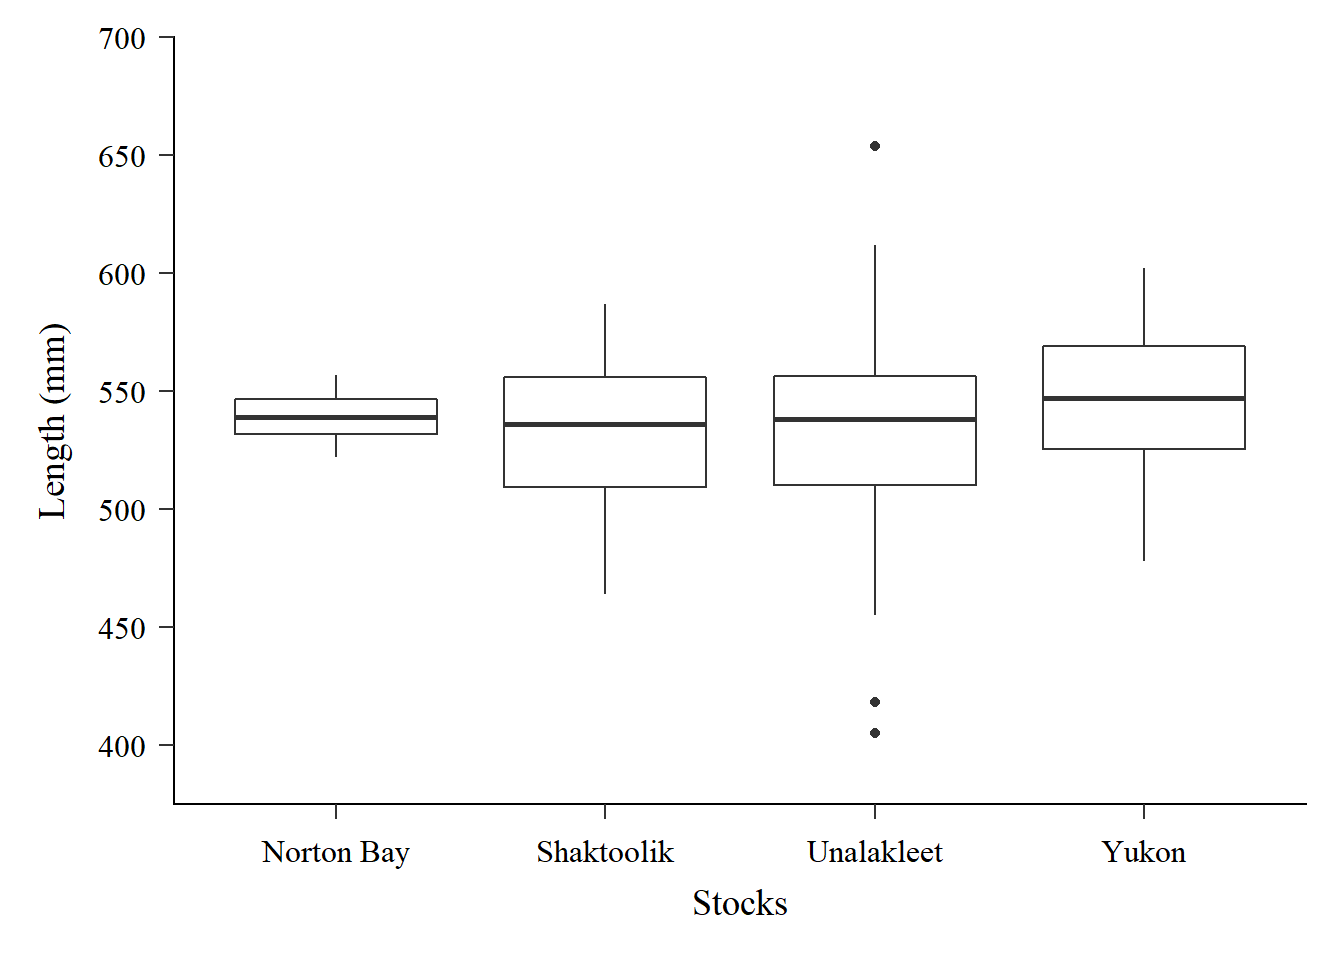
\includegraphics{Lab-5-Linear-Models_files/figure-latex/unnamed-chunk-2-1.pdf}

Looks pretty good! The relationship is now at least approximately linear
and there is no evidence of unequal variances (that is, the vertical
spread of the y-values is about the same over the range of x-values!!
Seems like regression assumptions would probably be met if we fit a
simple linear regression to the data. We can write the model as folows:

\begin{quote}
Model: \(log(brain) = a + b * log(body) + \epsilon\)
\end{quote}

To fit the model, you can simply replace \texttt{plot} in the above
expression with \texttt{lm}:

\begin{Shaded}
\begin{Highlighting}[]
\NormalTok{mammals.lm }\OtherTok{\textless{}{-}} \FunctionTok{lm}\NormalTok{(}\FunctionTok{log}\NormalTok{(brain)}\SpecialCharTok{\textasciitilde{}}\FunctionTok{log}\NormalTok{(body), }\AttributeTok{data=}\NormalTok{mammals)}
\end{Highlighting}
\end{Shaded}

The output from the model, including regression statistics, fitted
values, residuals and other values are stored in the resulting object
\texttt{mammals.lm} We start by extracting a basic summary of the
regression results from the fitted model object. Remeber that the
\texttt{summary} function checks the class of the object and then uses
the \texttt{summary.lm} method to do something sensible with the
contents of \texttt{mammals.lm}, in this case producing the following:

\begin{Shaded}
\begin{Highlighting}[]
\FunctionTok{summary}\NormalTok{(mammals.lm)}
\end{Highlighting}
\end{Shaded}

\begin{verbatim}
## 
## Call:
## lm(formula = log(brain) ~ log(body), data = mammals)
## 
## Residuals:
##      Min       1Q   Median       3Q      Max 
## -1.71550 -0.49228 -0.06162  0.43597  1.94829 
## 
## Coefficients:
##             Estimate Std. Error t value Pr(>|t|)    
## (Intercept)  2.13479    0.09604   22.23   <2e-16 ***
## log(body)    0.75169    0.02846   26.41   <2e-16 ***
## ---
## Signif. codes:  0 '***' 0.001 '**' 0.01 '*' 0.05 '.' 0.1 ' ' 1
## 
## Residual standard error: 0.6943 on 60 degrees of freedom
## Multiple R-squared:  0.9208, Adjusted R-squared:  0.9195 
## F-statistic: 697.4 on 1 and 60 DF,  p-value: < 2.2e-16
\end{verbatim}

As we saw before, the fitted model object is a list of various
components:

\begin{Shaded}
\begin{Highlighting}[]
\FunctionTok{names}\NormalTok{(mammals.lm)   }
\end{Highlighting}
\end{Shaded}

\begin{verbatim}
##  [1] "coefficients"  "residuals"     "effects"       "rank"         
##  [5] "fitted.values" "assign"        "qr"            "df.residual"  
##  [9] "xlevels"       "call"          "terms"         "model"
\end{verbatim}

We can extract individual components using the \$ notation and the
appropriate names (note that you don't have to type the full name, only
enough to uniquely identify the component):

\begin{Shaded}
\begin{Highlighting}[]
\NormalTok{mammals.lm}\SpecialCharTok{$}\NormalTok{call     }\CommentTok{\# the code that we can type to create this model}
\NormalTok{mammals.lm}\SpecialCharTok{$}\NormalTok{coef     }\CommentTok{\# parameter estimates (regression coefficients)}
\NormalTok{mammals.lm}\SpecialCharTok{$}\NormalTok{fit      }\CommentTok{\# fitted values}
\NormalTok{mammals.lm}\SpecialCharTok{$}\NormalTok{res      }\CommentTok{\# residuals}
\NormalTok{mammals.lm}\SpecialCharTok{$}\NormalTok{rank     }\CommentTok{\# number of parameters estimated (p=model degrees of freedom)}
\NormalTok{mammals.lm}\SpecialCharTok{$}\NormalTok{df.res   }\CommentTok{\# residual degrees of freedom (=n{-}p)}
\end{Highlighting}
\end{Shaded}

Some of these components can instead be extracted using the
corresponding generic ``extractor'' functions (preferred):

\begin{Shaded}
\begin{Highlighting}[]
\FunctionTok{coef}\NormalTok{(mammals.lm)        }\CommentTok{\# same as:  mammals.lm$coef}
\FunctionTok{fitted}\NormalTok{(mammals.lm)  }\CommentTok{\# same as: mammals.lm$fitted}
\FunctionTok{residuals}\NormalTok{(mammals.lm)   }\CommentTok{\# same as: mammals.lm$resid}
\CommentTok{\# selects one of five different kinds of residuals}
\FunctionTok{resid}\NormalTok{(mammals.lm, }\AttributeTok{type=}\StringTok{"pearson"}\NormalTok{)       }\CommentTok{\# short alias for \textquotesingle{}residuals\textquotesingle{}}
\end{Highlighting}
\end{Shaded}

Similar to the fitted model object itself (\texttt{mammals.lm}), the
\texttt{summary} function results in another list that contains various
components. Let's explore the components of the summary object (as
computed by \texttt{summary}):

\begin{Shaded}
\begin{Highlighting}[]
\FunctionTok{names}\NormalTok{(}\FunctionTok{summary}\NormalTok{(mammals.lm))       }\CommentTok{\# Components of the summary object}
\end{Highlighting}
\end{Shaded}

\begin{verbatim}
##  [1] "call"          "terms"         "residuals"     "coefficients" 
##  [5] "aliased"       "sigma"         "df"            "r.squared"    
##  [9] "adj.r.squared" "fstatistic"    "cov.unscaled"
\end{verbatim}

\begin{Shaded}
\begin{Highlighting}[]
\FunctionTok{summary}\NormalTok{(mammals.lm)}\SpecialCharTok{$}\NormalTok{coef         }\CommentTok{\# Table of \textquotesingle{}coefficients\textquotesingle{} with std errors, etc}
\end{Highlighting}
\end{Shaded}

\begin{verbatim}
##              Estimate Std. Error  t value     Pr(>|t|)
## (Intercept) 2.1347887 0.09604339 22.22734 1.183207e-30
## log(body)   0.7516859 0.02846356 26.40871 9.835792e-35
\end{verbatim}

For further computations, it typically makes sense to save the output
from a call to summary, then extract the components that you need:

\begin{Shaded}
\begin{Highlighting}[]
\NormalTok{s }\OtherTok{\textless{}{-}} \FunctionTok{summary}\NormalTok{(mammals.lm)}
\NormalTok{s}\SpecialCharTok{$}\NormalTok{coe       }\CommentTok{\# parameter estimates with std. errors and t test (Hyp: coef=0)}
\end{Highlighting}
\end{Shaded}

\begin{verbatim}
##              Estimate Std. Error  t value     Pr(>|t|)
## (Intercept) 2.1347887 0.09604339 22.22734 1.183207e-30
## log(body)   0.7516859 0.02846356 26.40871 9.835792e-35
\end{verbatim}

\begin{Shaded}
\begin{Highlighting}[]
\NormalTok{s}\SpecialCharTok{$}\NormalTok{r.sq    }\CommentTok{\# R{-}square}
\end{Highlighting}
\end{Shaded}

\begin{verbatim}
## [1] 0.9207837
\end{verbatim}

\begin{Shaded}
\begin{Highlighting}[]
\NormalTok{s}\SpecialCharTok{$}\NormalTok{fstat   }\CommentTok{\# F{-}statistic (\textquotesingle{}value\textquotesingle{}) with numerator and denominator d.f.}
\end{Highlighting}
\end{Shaded}

\begin{verbatim}
##  value  numdf  dendf 
## 697.42   1.00  60.00
\end{verbatim}

To simplify the code below, we save the independent (explanatory) and
dependent (response) variable as vectors `x' and `y', respectively:

\begin{Shaded}
\begin{Highlighting}[]
\NormalTok{x }\OtherTok{\textless{}{-}} \FunctionTok{log}\NormalTok{(mammals}\SpecialCharTok{$}\NormalTok{body)}
\NormalTok{y }\OtherTok{\textless{}{-}} \FunctionTok{log}\NormalTok{(mammals}\SpecialCharTok{$}\NormalTok{brain)}
\end{Highlighting}
\end{Shaded}

We start by fitting the ``null model'', that is a model that fits an
intercept only (with zero slope, i.e.~a horizontal line through the
data):

\begin{Shaded}
\begin{Highlighting}[]
\NormalTok{fit0 }\OtherTok{\textless{}{-}} \FunctionTok{lm}\NormalTok{(y }\SpecialCharTok{\textasciitilde{}} \DecValTok{1}\NormalTok{)}
\FunctionTok{summary}\NormalTok{(fit0)}
\end{Highlighting}
\end{Shaded}

\begin{verbatim}
## 
## Call:
## lm(formula = y ~ 1)
## 
## Residuals:
##     Min      1Q  Median      3Q     Max 
## -5.1063 -1.6981 -0.2925  1.9713  5.5101 
## 
## Coefficients:
##             Estimate Std. Error t value Pr(>|t|)    
## (Intercept)   3.1402     0.3107   10.11 1.19e-14 ***
## ---
## Signif. codes:  0 '***' 0.001 '**' 0.01 '*' 0.05 '.' 0.1 ' ' 1
## 
## Residual standard error: 2.447 on 61 degrees of freedom
\end{verbatim}

The null model is simply estimating the mean (and variance or standard
deviation) of the y-values:

\begin{Shaded}
\begin{Highlighting}[]
\FunctionTok{mean}\NormalTok{(y); }\FunctionTok{sd}\NormalTok{(y)  }
\end{Highlighting}
\end{Shaded}

\begin{verbatim}
## [1] 3.140198
\end{verbatim}

\begin{verbatim}
## [1] 2.446512
\end{verbatim}

Compare the mean and standard deviation of the y-values to the intercept
and the residual standard error estimated by the null model! Obviously,
this is not a very sensible model as there is a clear relationship
between brain size and body size, but the model is useful for comparison
purposes.

A reasonable assumption may be that the relationship between brain size
and body size goes through the origin (i.e.log-brain size decreases
linearly with log-body size and approaches zero when body size
approaches zero). We can force the line to go through the origin by
removing the intercept using `-1'. This estimates a slope only, but no
intercept:

\begin{Shaded}
\begin{Highlighting}[]
\NormalTok{fit.slope }\OtherTok{\textless{}{-}} \FunctionTok{lm}\NormalTok{(y }\SpecialCharTok{\textasciitilde{}}\NormalTok{ x }\SpecialCharTok{{-}} \DecValTok{1}\NormalTok{)}
\end{Highlighting}
\end{Shaded}

Plotting the results suggests a very poor fit:

\begin{Shaded}
\begin{Highlighting}[]
\FunctionTok{plot}\NormalTok{(x, y, }\AttributeTok{xlim=}\FunctionTok{c}\NormalTok{(}\DecValTok{0}\NormalTok{,}\FunctionTok{max}\NormalTok{(x)), }\AttributeTok{ylim=}\FunctionTok{c}\NormalTok{(}\DecValTok{0}\NormalTok{,}\FunctionTok{max}\NormalTok{(y))); }\FunctionTok{abline}\NormalTok{(fit.slope)}
\end{Highlighting}
\end{Shaded}

\includegraphics{Lab-5-Linear-Models_files/figure-latex/unnamed-chunk-14-1.pdf}

What does this imply about the brain-body size relationship? The poor
fit suggests that we should definitely include an intercept, hence we
fit a simple linear regression (same as `mammals.lm' above):

\begin{Shaded}
\begin{Highlighting}[]
\NormalTok{fit1 }\OtherTok{\textless{}{-}} \FunctionTok{lm}\NormalTok{(y }\SpecialCharTok{\textasciitilde{}}\NormalTok{ x)}
\FunctionTok{summary}\NormalTok{(fit1)       }
\end{Highlighting}
\end{Shaded}

\begin{verbatim}
## 
## Call:
## lm(formula = y ~ x)
## 
## Residuals:
##      Min       1Q   Median       3Q      Max 
## -1.71550 -0.49228 -0.06162  0.43597  1.94829 
## 
## Coefficients:
##             Estimate Std. Error t value Pr(>|t|)    
## (Intercept)  2.13479    0.09604   22.23   <2e-16 ***
## x            0.75169    0.02846   26.41   <2e-16 ***
## ---
## Signif. codes:  0 '***' 0.001 '**' 0.01 '*' 0.05 '.' 0.1 ' ' 1
## 
## Residual standard error: 0.6943 on 60 degrees of freedom
## Multiple R-squared:  0.9208, Adjusted R-squared:  0.9195 
## F-statistic: 697.4 on 1 and 60 DF,  p-value: < 2.2e-16
\end{verbatim}

This regression explains 92\% of the variability in brain size using
body size as a predictor (both on the log-scale, of course). Not bad! We
can formally compare the simple liner regression to the null model using
an F-test. The F-test (as well as other tests) is implemented in the
`anova' function that can be used to compare models, as well as test the
overall fit of a model:

\begin{Shaded}
\begin{Highlighting}[]
\FunctionTok{anova}\NormalTok{(fit0, fit1)       }\CommentTok{\# Compare two model fits using F{-}test}
\end{Highlighting}
\end{Shaded}

\begin{verbatim}
## Analysis of Variance Table
## 
## Model 1: y ~ 1
## Model 2: y ~ x
##   Res.Df    RSS Df Sum of Sq      F    Pr(>F)    
## 1     61 365.11                                  
## 2     60  28.92  1    336.19 697.42 < 2.2e-16 ***
## ---
## Signif. codes:  0 '***' 0.001 '**' 0.01 '*' 0.05 '.' 0.1 ' ' 1
\end{verbatim}

The F-test compares the residual sum of squares (RSS) of the ``bigger''
model (the simple linear regression - Model 2) to the RSS of the smaller
model (the null model - Model 1) and assesses whether the bigger model
reduces RSS enough to justify the extra parameter or whether you could
achieve the observed reduction in RSS by chance alone even if the null
model is true. In this case, there is overwhelming evidence (p
\textless\textless{} 0) that the simple linear regression provides a
better fit to the data (that is, we can reject the null model
decisively).

We may also want to test if brain size is linearly proportional to body
size or if there is evidence that brain size levels off as body size
increases (on the log scale - we already saw that this is true on the
`raw' scale, hence we did a log-transformation in the first place).

If there is curvature on the log-scale, this should be evident in a
significant curvature in the relationship, which we can estimate (for
example) by adding a quadratic term to the model:

\begin{quote}
Quadratic model: \(y = a + b_{1} * x + b_2 * x^{2} + \epsilon\)
\end{quote}

In R notation, we need to use the identity function `I' - which simply
returns the values for \(x^{2}\) - to fit the quadratic model
(otherwise, R will interpret `\^{}' as part of the model formula,
denoting `expansion' of terms. We can fit the new model using the
`update' function, which means that R does not have to refit the entire
model as it uses the old output (although the computational savings are
trivial here). The output shows the full fitted model (Component
`Call').

\begin{Shaded}
\begin{Highlighting}[]
\NormalTok{fit2 }\OtherTok{\textless{}{-}} \FunctionTok{update}\NormalTok{(fit1, }\SpecialCharTok{\textasciitilde{}}\NormalTok{ . }\SpecialCharTok{+} \FunctionTok{I}\NormalTok{(x}\SpecialCharTok{\^{}}\DecValTok{2}\NormalTok{))   }
\FunctionTok{summary}\NormalTok{(fit2)}
\end{Highlighting}
\end{Shaded}

\begin{verbatim}
## 
## Call:
## lm(formula = y ~ x + I(x^2))
## 
## Residuals:
##      Min       1Q   Median       3Q      Max 
## -1.78339 -0.48897 -0.03167  0.40117  1.92624 
## 
## Coefficients:
##              Estimate Std. Error t value Pr(>|t|)    
## (Intercept)  2.185905   0.109917  19.887   <2e-16 ***
## x            0.773983   0.036777  21.045   <2e-16 ***
## I(x^2)      -0.007109   0.007418  -0.958    0.342    
## ---
## Signif. codes:  0 '***' 0.001 '**' 0.01 '*' 0.05 '.' 0.1 ' ' 1
## 
## Residual standard error: 0.6948 on 59 degrees of freedom
## Multiple R-squared:  0.922,  Adjusted R-squared:  0.9194 
## F-statistic: 348.7 on 2 and 59 DF,  p-value: < 2.2e-16
\end{verbatim}

What does that say about any curvature? We can look at the coefficient
for the quadratic term and check if it is significantly different from
zero. That's exactly what the ``t-test'' in the output does. It always
tests whether the estimated coefficient is significantly different from
zero (null hypothesis), whether that is sensible or not. In this case it
means that the quadratic term is not significant, hence the simpler
model is preferable.

Equivalently, we can compare the simple linear regression with the
quadratic regression by comparing the nested models using an F-test:

\begin{Shaded}
\begin{Highlighting}[]
\FunctionTok{anova}\NormalTok{(fit1, fit2)}
\end{Highlighting}
\end{Shaded}

\begin{verbatim}
## Analysis of Variance Table
## 
## Model 1: y ~ x
## Model 2: y ~ x + I(x^2)
##   Res.Df    RSS Df Sum of Sq      F Pr(>F)
## 1     60 28.923                           
## 2     59 28.479  1   0.44335 0.9185 0.3418
\end{verbatim}

Note that the p-value for comparing the simple linear and quadratic
regressions is identical in this case to the p-value from the t-test for
the quadratic term!

Conclusion: We cannot reject the null hypothesis that the simple linear
regression is the ``true'' model (i.e.~that the coefficient for the
quadratic term is zero). Hence the data do not provide evidence of
curvi-linearity in the relationship between the logarithm of body size
and the logarithm of brain size!

As an alternative to fitting the linear and quadratic terms as two
separate terms, we can also fit the full quadratic model using poly(),
which is the preferred approach:

\begin{Shaded}
\begin{Highlighting}[]
\NormalTok{fit }\OtherTok{\textless{}{-}} \FunctionTok{lm}\NormalTok{(y }\SpecialCharTok{\textasciitilde{}} \FunctionTok{poly}\NormalTok{(x, }\DecValTok{2}\NormalTok{))}
\end{Highlighting}
\end{Shaded}

Essentially, \texttt{poly()} creates two new variables that are
equivalent to the linear and quadratic terms but are not correlated with
each other. Note that \(x\) and \(x^{2}\) are highly correlated with
each other (r = 0.6326107), whereas the two new variables are not:

\begin{Shaded}
\begin{Highlighting}[]
\NormalTok{new }\OtherTok{\textless{}{-}} \FunctionTok{poly}\NormalTok{(x, }\DecValTok{2}\NormalTok{)}
\FunctionTok{head}\NormalTok{(new)              }\CommentTok{\# New, rotated variables}
\end{Highlighting}
\end{Shaded}

\begin{verbatim}
##                 1           2
## [1,] -0.004845158 -0.10172760
## [2,] -0.084924303 -0.04643912
## [3,] -0.042531038 -0.08585726
## [4,]  0.196966969  0.12032199
## [5,]  0.092451101 -0.05927273
## [6,]  0.081273175 -0.07026520
\end{verbatim}

These are rotated versions of the original \(x\) and \(x^{2}\) terms
(linear rotations) which are uncorrelated with each other, as you can
easily see:

\begin{Shaded}
\begin{Highlighting}[]
\FunctionTok{cor}\NormalTok{(}\FunctionTok{poly}\NormalTok{(x,}\DecValTok{2}\NormalTok{))}
\end{Highlighting}
\end{Shaded}

\begin{verbatim}
##             1           2
## 1 1.00000e+00 4.81092e-17
## 2 4.81092e-17 1.00000e+00
\end{verbatim}

Comparing the fit with \texttt{poly} to the original quadratic fit
(\texttt{fit2}), we see that the estimated coefficients are very
different because the independent variables are different (different
``parameterization''"). However, the fitted values are identical, as
evident in the plot:

\begin{Shaded}
\begin{Highlighting}[]
\FunctionTok{coef}\NormalTok{(fit)}
\end{Highlighting}
\end{Shaded}

\begin{verbatim}
## (Intercept) poly(x, 2)1 poly(x, 2)2 
##    3.140198   18.335429   -0.665842
\end{verbatim}

\begin{Shaded}
\begin{Highlighting}[]
\FunctionTok{coef}\NormalTok{(fit2)}
\end{Highlighting}
\end{Shaded}

\begin{verbatim}
##  (Intercept)            x       I(x^2) 
##  2.185904832  0.773983039 -0.007108917
\end{verbatim}

\begin{Shaded}
\begin{Highlighting}[]
\FunctionTok{plot}\NormalTok{(}\FunctionTok{fitted}\NormalTok{(fit), }\FunctionTok{fitted}\NormalTok{(fit2))}
\FunctionTok{abline}\NormalTok{(}\DecValTok{0}\NormalTok{,}\DecValTok{1}\NormalTok{)        }\CommentTok{\# Add line with intercept 0, slope 1 (1:1 correspondence line)}
\end{Highlighting}
\end{Shaded}

\includegraphics{Lab-5-Linear-Models_files/figure-latex/unnamed-chunk-22-1.pdf}

The fits are completely identical - the only difference is that poly()
uses a ``better'' parameterization in which parameters are uncorrelated
(no multicollinearity issues!).

We can visualize the model fit using, for example, the `termplot'
function (see help file for info!). It returns a single fitted
relationship for the quadratic (`poly') term that shows the estimated
relationship:

\begin{Shaded}
\begin{Highlighting}[]
\FunctionTok{termplot}\NormalTok{(fit, }\AttributeTok{se=}\NormalTok{T, }\AttributeTok{partial.resid=}\NormalTok{T)}
\end{Highlighting}
\end{Shaded}

\includegraphics{Lab-5-Linear-Models_files/figure-latex/unnamed-chunk-23-1.pdf}

There is slight curvature in the estimated fit, but as we saw above it
is not signifcant and a linear models should be adequate!

Now let's take a closer look at humans to examine if we have an unusual
brain size!

\begin{Shaded}
\begin{Highlighting}[]
\FunctionTok{plot}\NormalTok{(}\FunctionTok{log}\NormalTok{(mammals}\SpecialCharTok{$}\NormalTok{body), }\FunctionTok{log}\NormalTok{(mammals}\SpecialCharTok{$}\NormalTok{brain))}
\FunctionTok{abline}\NormalTok{(mammals.lm)      }\CommentTok{\# Add regression line}

\CommentTok{\# Extract values for humans from data frame and log{-}transform, then highlight humans in plot: }
\NormalTok{human }\OtherTok{\textless{}{-}} \FunctionTok{log}\NormalTok{(mammals[}\StringTok{"Human"}\NormalTok{, ])}
\NormalTok{human}
\end{Highlighting}
\end{Shaded}

\begin{verbatim}
##           body    brain
## Human 4.127134 7.185387
\end{verbatim}

\begin{Shaded}
\begin{Highlighting}[]
\FunctionTok{points}\NormalTok{(human[}\DecValTok{1}\NormalTok{], human[}\DecValTok{2}\NormalTok{], }\AttributeTok{pch=}\DecValTok{16}\NormalTok{, }\AttributeTok{cex=}\DecValTok{2}\NormalTok{, }\AttributeTok{col =} \DecValTok{2}\NormalTok{)}
\FunctionTok{text}\NormalTok{(human[}\DecValTok{1}\NormalTok{], human[}\DecValTok{2}\NormalTok{]}\SpecialCharTok{+}\DecValTok{1}\NormalTok{, }\StringTok{"me"}\NormalTok{, }\AttributeTok{cex=}\DecValTok{2}\NormalTok{)}
\end{Highlighting}
\end{Shaded}

\includegraphics{Lab-5-Linear-Models_files/figure-latex/unnamed-chunk-24-1.pdf}

As should be obvious from this plot, we have an unusually large brain
size for our body size because the point is well above the regression
line!

Often, the purpose of this kind of regression is to make predictions. In
this case, we might want to predict the brain weights of other mammals
that were not included in the analysis and for which we may not have any
data. Let's predicts brain weight for three species weighing on average
60, 500 and 2000kg and add the predicted values to the plot. The
`predict' function works with most model functions and uses the fitted
model to predict the values of the response variable (log(brain weight))
at new values of the explanatory variables. The new values are specified
as a data frame with a variable name that has to match the name in the
model fit (`mammals.lm'). The new data are specified on the original
scale because the log-transformation is done in the model formula.

\begin{Shaded}
\begin{Highlighting}[]
\NormalTok{pred }\OtherTok{\textless{}{-}} \FunctionTok{predict}\NormalTok{(mammals.lm, }\AttributeTok{newdata=}\FunctionTok{data.frame}\NormalTok{(}\AttributeTok{body=}\FunctionTok{c}\NormalTok{(}\DecValTok{60}\NormalTok{, }\DecValTok{500}\NormalTok{, }\DecValTok{2000}\NormalTok{)))}
\FunctionTok{plot}\NormalTok{(}\FunctionTok{log}\NormalTok{(mammals}\SpecialCharTok{$}\NormalTok{body), }\FunctionTok{log}\NormalTok{(mammals}\SpecialCharTok{$}\NormalTok{brain))}
\FunctionTok{abline}\NormalTok{(mammals.lm)      }\CommentTok{\# Add regression line}
\FunctionTok{points}\NormalTok{(}\FunctionTok{log}\NormalTok{(}\FunctionTok{c}\NormalTok{(}\DecValTok{60}\NormalTok{, }\DecValTok{500}\NormalTok{,}\DecValTok{2000}\NormalTok{)), pred, }\AttributeTok{pch=}\DecValTok{16}\NormalTok{, }\AttributeTok{cex=}\DecValTok{2}\NormalTok{, }\AttributeTok{col=}\DecValTok{3}\NormalTok{)}
\end{Highlighting}
\end{Shaded}

The difference is much more pronounced on the back-transformed (`raw')
scale! We can back-transform the predicted values, which were computed
on the log scale (x), by exponentiating (i.e.~the inverse of taking the
log):

\begin{Shaded}
\begin{Highlighting}[]
\FunctionTok{plot}\NormalTok{(mammals}\SpecialCharTok{$}\NormalTok{body, mammals}\SpecialCharTok{$}\NormalTok{brain)}
\FunctionTok{points}\NormalTok{(}\FunctionTok{c}\NormalTok{(}\DecValTok{60}\NormalTok{,}\DecValTok{500}\NormalTok{,}\DecValTok{2000}\NormalTok{), }\FunctionTok{exp}\NormalTok{(pred), }\AttributeTok{pch=}\DecValTok{16}\NormalTok{, }\AttributeTok{cex=}\DecValTok{3}\NormalTok{, }\AttributeTok{col=}\DecValTok{3}\NormalTok{)}
\end{Highlighting}
\end{Shaded}

Note that this corresponds to the predicted \textbf{median} brain size
at a given body size, NOT the predicted \textbf{mean} brain size. To
compute mean brain size at a given body size we would need to apply a
bias correction when converting from the log-scale back to the original
scale (using \(exp(x + s^{2}/2)\), where \(s^{2}\) is the estimated
residual variance).

\hypertarget{exercise}{%
\subsection{Exercise}\label{exercise}}

Plot the fitted relationship between body size and brain size on the raw
(untransformed) scale by (1) creating a vector of ordered,
equally-spaced body sizes (x-values) spanning the range of observed body
sizes, (2) computing predicted brain sizes for these x values on the
log-scale, (3) back-transforming the predicted values to compute median
or mean brain size at a given body size, and (4) adding the results as a
line on a scatterplot of the data.

\hypertarget{diagnostics}{%
\subsection{Diagnostics}\label{diagnostics}}

Whenever you fit a model, you should run some basic diagnostics:

\begin{Shaded}
\begin{Highlighting}[]
\FunctionTok{par}\NormalTok{(}\AttributeTok{mfrow=}\FunctionTok{c}\NormalTok{(}\DecValTok{2}\NormalTok{,}\DecValTok{2}\NormalTok{))}
\FunctionTok{plot}\NormalTok{(mammals.lm)        }\CommentTok{\# Do you find any unusual patterns? Outliers?}
\end{Highlighting}
\end{Shaded}

\includegraphics{Lab-5-Linear-Models_files/figure-latex/unnamed-chunk-27-1.pdf}

\begin{Shaded}
\begin{Highlighting}[]
\FunctionTok{par}\NormalTok{(}\AttributeTok{mfrow=}\FunctionTok{c}\NormalTok{(}\DecValTok{1}\NormalTok{,}\DecValTok{1}\NormalTok{))}
\end{Highlighting}
\end{Shaded}

There are no obvious patterns that would be of concern in the plot and
the data are close to normally distributed. Quite often, we may want to
know what observation a particular point in a diagnostic plot
corresponds to. To identify any unusual / extreme values interactively,
you can use the `identify' function:

\begin{Shaded}
\begin{Highlighting}[]
\FunctionTok{plot}\NormalTok{(mammals.lm}\SpecialCharTok{$}\NormalTok{fit, mammals.lm}\SpecialCharTok{$}\NormalTok{res)}
\FunctionTok{abline}\NormalTok{(}\AttributeTok{h=}\DecValTok{0}\NormalTok{)}
\FunctionTok{identify}\NormalTok{(mammals.lm}\SpecialCharTok{$}\NormalTok{fit, mammals.lm}\SpecialCharTok{$}\NormalTok{res, }\FunctionTok{row.names}\NormalTok{(mammals))}
\end{Highlighting}
\end{Shaded}

This puts you in interactive mode and you can click near data points to
label the point with the name of the mammal (which \texttt{identify}
gets from the row names). Click on one or more points and hit escape
when done, which adds labels to the points!

As measured by the magnitude of the residual (i.e.~the distance from the
average brain size at a given body size), who is the ``smartest'' of
them all? Who is apparently the ``dumbest'' mammal by this measure?

Let's remove humans and re-fit the model. To do so, we can create a
logical vector that is true for all rows in \texttt{mammals} except for
the row corresponding to humans. We then update the model for the subset
that does not include humans:

\begin{Shaded}
\begin{Highlighting}[]
\NormalTok{(j }\OtherTok{\textless{}{-}} \FunctionTok{row.names}\NormalTok{(mammals) }\SpecialCharTok{!=} \StringTok{"Human"}\NormalTok{)}
\end{Highlighting}
\end{Shaded}

\begin{verbatim}
##  [1]  TRUE  TRUE  TRUE  TRUE  TRUE  TRUE  TRUE  TRUE  TRUE  TRUE  TRUE  TRUE
## [13]  TRUE  TRUE  TRUE  TRUE  TRUE  TRUE  TRUE  TRUE  TRUE  TRUE  TRUE  TRUE
## [25]  TRUE  TRUE  TRUE  TRUE  TRUE  TRUE  TRUE FALSE  TRUE  TRUE  TRUE  TRUE
## [37]  TRUE  TRUE  TRUE  TRUE  TRUE  TRUE  TRUE  TRUE  TRUE  TRUE  TRUE  TRUE
## [49]  TRUE  TRUE  TRUE  TRUE  TRUE  TRUE  TRUE  TRUE  TRUE  TRUE  TRUE  TRUE
## [61]  TRUE  TRUE
\end{verbatim}

\begin{Shaded}
\begin{Highlighting}[]
\NormalTok{mammals.lm2 }\OtherTok{\textless{}{-}} \FunctionTok{update}\NormalTok{(mammals.lm, }\AttributeTok{subset =}\NormalTok{ j)}
\end{Highlighting}
\end{Shaded}

Let's compare the fitted lines and parameter estimates to the model with
all data included:

\begin{Shaded}
\begin{Highlighting}[]
\FunctionTok{plot}\NormalTok{(}\FunctionTok{log}\NormalTok{(mammals}\SpecialCharTok{$}\NormalTok{body), }\FunctionTok{log}\NormalTok{(mammals}\SpecialCharTok{$}\NormalTok{brain))}
\FunctionTok{abline}\NormalTok{(mammals.lm)                }\CommentTok{\# Original fit    }
\FunctionTok{abline}\NormalTok{(mammals.lm2, }\AttributeTok{col=}\DecValTok{2}\NormalTok{)      }\CommentTok{\# Fit after removing humans}
\end{Highlighting}
\end{Shaded}

\includegraphics{Lab-5-Linear-Models_files/figure-latex/unnamed-chunk-30-1.pdf}

The two fits are barely distinguishable in the plot!

\begin{Shaded}
\begin{Highlighting}[]
\FunctionTok{summary}\NormalTok{(mammals.lm)}\SpecialCharTok{$}\NormalTok{coef}
\end{Highlighting}
\end{Shaded}

\begin{verbatim}
##              Estimate Std. Error  t value     Pr(>|t|)
## (Intercept) 2.1347887 0.09604339 22.22734 1.183207e-30
## log(body)   0.7516859 0.02846356 26.40871 9.835792e-35
\end{verbatim}

\begin{Shaded}
\begin{Highlighting}[]
\FunctionTok{summary}\NormalTok{(mammals.lm2)}\SpecialCharTok{$}\NormalTok{coef}
\end{Highlighting}
\end{Shaded}

\begin{verbatim}
##              Estimate Std. Error  t value     Pr(>|t|)
## (Intercept) 2.1150046 0.09030476 23.42074 1.448627e-31
## log(body)   0.7422766 0.02687233 27.62233 1.913452e-35
\end{verbatim}

We can compute the change in coefficients when eliminating humans from
the regression. This is a diagnostic measure that quantifies the
``influence'' of humans on the regression:

\begin{Shaded}
\begin{Highlighting}[]
\FunctionTok{coef}\NormalTok{(mammals.lm) }\SpecialCharTok{{-}} \FunctionTok{coef}\NormalTok{(mammals.lm2)}
\end{Highlighting}
\end{Shaded}

\begin{verbatim}
## (Intercept)   log(body) 
## 0.019784111 0.009409341
\end{verbatim}

The difference seems fairly small. You can easily compute the change in
coefficients that results from dropping each observation in turn using
the `influence' function:

\begin{Shaded}
\begin{Highlighting}[]
\NormalTok{mammals.infl }\OtherTok{\textless{}{-}} \FunctionTok{influence}\NormalTok{(mammals.lm)}

\CommentTok{\# Change in coefficients after dropping humans (compare to results above!):}
\NormalTok{mammals.infl}\SpecialCharTok{$}\NormalTok{coeff[}\StringTok{"Human"}\NormalTok{, ]}
\end{Highlighting}
\end{Shaded}

\begin{verbatim}
## (Intercept)   log(body) 
## 0.019784111 0.009409341
\end{verbatim}

\begin{Shaded}
\begin{Highlighting}[]
\CommentTok{\# Change in coefficients for dropping any given observation (only first 5 are shown):}
\FunctionTok{head}\NormalTok{(mammals.infl}\SpecialCharTok{$}\NormalTok{coeff)}
\end{Highlighting}
\end{Shaded}

\begin{verbatim}
##                   (Intercept)     log(body)
## Arctic fox       0.0124000790 -0.0001502360
## Owl monkey       0.0246402067 -0.0041271962
## Mountain beaver -0.0050475381  0.0004767287
## Cow             -0.0039709654 -0.0060176918
## Grey wolf       -0.0005897846 -0.0002021220
## Goat             0.0013682552  0.0003905679
\end{verbatim}

We checked for a specific form of curvature (`quadratic') when we fit
the quadratic model. Maybe the relationship is non-linear in some other
way? For example, we can fit a more flexible non-parametric smooth
function that is commonly used to estimate relationships between a
predictor and a respons (LOWESS). The corresponding function is
\texttt{loess}, which uses the same formula structure as other modeling
functions and we can use some of the same extractor functions such as
\texttt{fitted} and \texttt{resid}. However, the fitted model has no
model coefficients, so \texttt{coef(mammals.loess)} results in
\texttt{NULL}

\begin{Shaded}
\begin{Highlighting}[]
\NormalTok{mammals.loess }\OtherTok{\textless{}{-}} \FunctionTok{loess}\NormalTok{(}\FunctionTok{log}\NormalTok{(brain)}\SpecialCharTok{\textasciitilde{}}\FunctionTok{log}\NormalTok{(body), }\AttributeTok{data=}\NormalTok{mammals)}
\NormalTok{mammals.loess}
\end{Highlighting}
\end{Shaded}

\begin{verbatim}
## Call:
## loess(formula = log(brain) ~ log(body), data = mammals)
## 
## Number of Observations: 62 
## Equivalent Number of Parameters: 5.02 
## Residual Standard Error: 0.6805
\end{verbatim}

\begin{Shaded}
\begin{Highlighting}[]
\FunctionTok{summary}\NormalTok{(mammals.loess)  }\CommentTok{\# Output is quite different from a linear model!}
\end{Highlighting}
\end{Shaded}

\begin{verbatim}
## Call:
## loess(formula = log(brain) ~ log(body), data = mammals)
## 
## Number of Observations: 62 
## Equivalent Number of Parameters: 5.02 
## Residual Standard Error: 0.6805 
## Trace of smoother matrix: 5.51  (exact)
## 
## Control settings:
##   span     :  0.75 
##   degree   :  2 
##   family   :  gaussian
##   surface  :  interpolate      cell = 0.2
##   normalize:  TRUE
##  parametric:  FALSE
## drop.square:  FALSE
\end{verbatim}

\begin{Shaded}
\begin{Highlighting}[]
\FunctionTok{names}\NormalTok{(mammals.loess)    }\CommentTok{\# Components of the model fit}
\end{Highlighting}
\end{Shaded}

\begin{verbatim}
##  [1] "n"         "fitted"    "residuals" "enp"       "s"         "one.delta"
##  [7] "two.delta" "trace.hat" "divisor"   "robust"    "pars"      "kd"       
## [13] "call"      "terms"     "xnames"    "x"         "y"         "weights"
\end{verbatim}

\begin{Shaded}
\begin{Highlighting}[]
\FunctionTok{fitted}\NormalTok{(mammals.loess)   }\CommentTok{\# Fitted values}
\FunctionTok{resid}\NormalTok{(mammals.loess)}
\end{Highlighting}
\end{Shaded}

\begin{Shaded}
\begin{Highlighting}[]
\CommentTok{\# Plot the fitted values on log{-}transformed scale:}
\FunctionTok{par}\NormalTok{(}\AttributeTok{mar=}\FunctionTok{c}\NormalTok{(}\DecValTok{5}\NormalTok{,}\DecValTok{4}\NormalTok{,}\DecValTok{1}\NormalTok{,}\DecValTok{1}\NormalTok{))}
\FunctionTok{plot}\NormalTok{(}\FunctionTok{log}\NormalTok{(mammals}\SpecialCharTok{$}\NormalTok{body), }\FunctionTok{fitted}\NormalTok{(mammals.loess), }\AttributeTok{col=}\DecValTok{6}\NormalTok{)}
\end{Highlighting}
\end{Shaded}

\includegraphics{Lab-5-Linear-Models_files/figure-latex/unnamed-chunk-36-1.pdf}

\begin{Shaded}
\begin{Highlighting}[]
\CommentTok{\# Or we can try to connect the fitted values with a line:}
\FunctionTok{par}\NormalTok{(}\AttributeTok{mar=}\FunctionTok{c}\NormalTok{(}\DecValTok{5}\NormalTok{,}\DecValTok{4}\NormalTok{,}\DecValTok{1}\NormalTok{,}\DecValTok{1}\NormalTok{))}
\FunctionTok{plot}\NormalTok{(}\FunctionTok{log}\NormalTok{(mammals}\SpecialCharTok{$}\NormalTok{body), }\FunctionTok{fitted}\NormalTok{(mammals.loess), }\AttributeTok{col=}\DecValTok{6}\NormalTok{)}
\FunctionTok{lines}\NormalTok{(}\FunctionTok{log}\NormalTok{(mammals}\SpecialCharTok{$}\NormalTok{body), }\FunctionTok{fitted}\NormalTok{(mammals.loess), }\AttributeTok{col=}\DecValTok{4}\NormalTok{)}
\end{Highlighting}
\end{Shaded}

\includegraphics{Lab-5-Linear-Models_files/figure-latex/unnamed-chunk-37-1.pdf}

OOPS! This creates a mess because the x-values are not sorted! We can
fix the plot by sorting values before connecting them with a line:

\begin{Shaded}
\begin{Highlighting}[]
\FunctionTok{par}\NormalTok{(}\AttributeTok{mar=}\FunctionTok{c}\NormalTok{(}\DecValTok{5}\NormalTok{,}\DecValTok{4}\NormalTok{,}\DecValTok{1}\NormalTok{,}\DecValTok{1}\NormalTok{))}
\NormalTok{x }\OtherTok{\textless{}{-}} \FunctionTok{log}\NormalTok{(mammals}\SpecialCharTok{$}\NormalTok{body)}
\NormalTok{y }\OtherTok{\textless{}{-}}\NormalTok{ mammals.loess}\SpecialCharTok{$}\NormalTok{fit}
\FunctionTok{plot}\NormalTok{(}\FunctionTok{log}\NormalTok{(mammals}\SpecialCharTok{$}\NormalTok{body), }\FunctionTok{log}\NormalTok{(mammals}\SpecialCharTok{$}\NormalTok{brain))}
\FunctionTok{lines}\NormalTok{(x[}\FunctionTok{order}\NormalTok{(x)], y[}\FunctionTok{order}\NormalTok{(x)])      }\CommentTok{\# In order of increasing x!}
\end{Highlighting}
\end{Shaded}

\includegraphics{Lab-5-Linear-Models_files/figure-latex/unnamed-chunk-38-1.pdf}

\pagebreak

\hypertarget{additional-material}{%
\subsection{Additional material}\label{additional-material}}

Here are some additional (optional) examples to explore and learn some
new regression tricks.

Let's explore another data set: the \texttt{cabbages} data from field
experiments First, learn about the data and take a look at it

\begin{Shaded}
\begin{Highlighting}[]
\NormalTok{?cabbages}
\FunctionTok{names}\NormalTok{(cabbages)}
\NormalTok{cabbages}
\end{Highlighting}
\end{Shaded}

Let's say we are interested in modeling the Vitamin C content to find
out what cabbages we should buy to maximize our Vitamin C intake. Or, in
other words, are there differences in Vitamin C content among varieties
(cultivar), by planting date, or by weight.

We'll start with some exploratory plots to get a feel for the data. I
dind't include any of the output to keep the clutter at bay and to
encourage you to explore on your own:

\begin{Shaded}
\begin{Highlighting}[]
\FunctionTok{library}\NormalTok{(lattice)}
\FunctionTok{dotplot}\NormalTok{(Date }\SpecialCharTok{\textasciitilde{}}\NormalTok{ VitC, }\AttributeTok{data=}\NormalTok{cabbages) }\CommentTok{\# Distribution of Vitamin C by date}
\FunctionTok{boxplot}\NormalTok{(cabbages}\SpecialCharTok{$}\NormalTok{VitC) }\CommentTok{\# Range and distribution of all Vitamin C values }

\CommentTok{\# Separate Vitamin C content by date, then plot their distribution by date:}
\NormalTok{VitC.by.date }\OtherTok{\textless{}{-}} \FunctionTok{split}\NormalTok{(cabbages}\SpecialCharTok{$}\NormalTok{VitC, cabbages}\SpecialCharTok{$}\NormalTok{Date)}
\FunctionTok{boxplot}\NormalTok{(VitC.by.date)}

\CommentTok{\# which is actually the same as: }
\FunctionTok{plot}\NormalTok{(cabbages}\SpecialCharTok{$}\NormalTok{Date, cabbages}\SpecialCharTok{$}\NormalTok{VitC)}

\CommentTok{\# Perhaps Vitamin C content various with weight ("head weight"):}
\FunctionTok{plot}\NormalTok{(VitC}\SpecialCharTok{\textasciitilde{}}\NormalTok{HeadWt, }\AttributeTok{data=}\NormalTok{cabbages)}
\FunctionTok{scatter.smooth}\NormalTok{(cabbages}\SpecialCharTok{$}\NormalTok{HeadWt, cabbages}\SpecialCharTok{$}\NormalTok{VitC) }

\CommentTok{\# The "scatter smooth" fits a LOWESS regression using loess and adds the result}
\CommentTok{\# to a scatter plot, hence is the same as:}
\FunctionTok{plot}\NormalTok{(VitC}\SpecialCharTok{\textasciitilde{}}\NormalTok{HeadWt, }\AttributeTok{data=}\NormalTok{cabbages)}
\NormalTok{(lo }\OtherTok{\textless{}{-}} \FunctionTok{loess.smooth}\NormalTok{(cabbages}\SpecialCharTok{$}\NormalTok{HeadWt, cabbages}\SpecialCharTok{$}\NormalTok{VitC)) }\CommentTok{\# Save output (predicted values)}
\FunctionTok{lines}\NormalTok{(lo) }\CommentTok{\# Add line to plot based on predicted values over range of x}

\CommentTok{\# Separate Vitamin C contents by cultivar, then plot:}
\FunctionTok{boxplot}\NormalTok{(}\FunctionTok{split}\NormalTok{(cabbages}\SpecialCharTok{$}\NormalTok{VitC, cabbages}\SpecialCharTok{$}\NormalTok{Cult))}

\CommentTok{\# Plot Vitamin C as a function of weight for different levels of Cult}
\FunctionTok{coplot}\NormalTok{(VitC}\SpecialCharTok{\textasciitilde{}}\NormalTok{HeadWt}\SpecialCharTok{|}\NormalTok{Cult, }\AttributeTok{data=}\NormalTok{cabbages)}

\CommentTok{\# Add scatterplot smoother (LOWESS smoother)}
\FunctionTok{coplot}\NormalTok{(VitC}\SpecialCharTok{\textasciitilde{}}\NormalTok{HeadWt}\SpecialCharTok{|}\NormalTok{Cult, }\AttributeTok{data=}\NormalTok{cabbages, }\AttributeTok{panel=}\NormalTok{panel.smooth)}

\CommentTok{\# Plot Vitamin C as a function of weight by date, with LOWESS smoother}
\FunctionTok{coplot}\NormalTok{(VitC}\SpecialCharTok{\textasciitilde{}}\NormalTok{HeadWt}\SpecialCharTok{|}\NormalTok{Date, }\AttributeTok{data=}\NormalTok{cabbages, }\AttributeTok{panel=}\NormalTok{panel.smooth, }\AttributeTok{rows=}\DecValTok{1}\NormalTok{)}

\CommentTok{\# Plot by date and Cult:}
\FunctionTok{coplot}\NormalTok{(VitC}\SpecialCharTok{\textasciitilde{}}\NormalTok{HeadWt}\SpecialCharTok{|}\NormalTok{Date}\SpecialCharTok{*}\NormalTok{Cult, }\AttributeTok{data=}\NormalTok{cabbages) }\CommentTok{\# OR, equivalently:}
\FunctionTok{coplot}\NormalTok{(VitC}\SpecialCharTok{\textasciitilde{}}\NormalTok{HeadWt}\SpecialCharTok{|}\NormalTok{Date}\SpecialCharTok{+}\NormalTok{Cult, }\AttributeTok{data=}\NormalTok{cabbages)}

\CommentTok{\# Exlore potential interactions between the two factors:}
\CommentTok{\# (Check help file: \textquotesingle{}?interaction.plot\textquotesingle{}}
\FunctionTok{attach}\NormalTok{(cabbages)}
\FunctionTok{interaction.plot}\NormalTok{(Cult, Date, VitC)}
\FunctionTok{interaction.plot}\NormalTok{(Date, Cult, VitC)}
\FunctionTok{detach}\NormalTok{(cabbages)}
\end{Highlighting}
\end{Shaded}

Now that we have explored the cabbages data, we'll fit some statistical
models to estimate if and how Vitamin C content varies among varieties,
by planting date, and with the weight of the cabbage.

For simplicity, we start with a two-way ANOVA, ignoring the obvious
influence of cabbage weight (for now):

\begin{Shaded}
\begin{Highlighting}[]
\NormalTok{cabbages.aov }\OtherTok{\textless{}{-}} \FunctionTok{aov}\NormalTok{(VitC}\SpecialCharTok{\textasciitilde{}}\NormalTok{Cult}\SpecialCharTok{+}\NormalTok{Date, }\AttributeTok{data=}\NormalTok{cabbages)}
\FunctionTok{summary}\NormalTok{(cabbages.aov)}
\end{Highlighting}
\end{Shaded}

\begin{verbatim}
##             Df Sum Sq Mean Sq F value   Pr(>F)    
## Cult         1 2496.1  2496.1  53.041 1.18e-09 ***
## Date         2  909.3   454.6   9.661 0.000249 ***
## Residuals   56 2635.4    47.1                     
## ---
## Signif. codes:  0 '***' 0.001 '**' 0.01 '*' 0.05 '.' 0.1 ' ' 1
\end{verbatim}

\begin{Shaded}
\begin{Highlighting}[]
\FunctionTok{par}\NormalTok{(}\AttributeTok{mfrow=}\FunctionTok{c}\NormalTok{(}\DecValTok{2}\NormalTok{,}\DecValTok{2}\NormalTok{))}
\FunctionTok{plot}\NormalTok{(cabbages.aov) }\CommentTok{\# Diagnostic plots}
\end{Highlighting}
\end{Shaded}

\includegraphics{Lab-5-Linear-Models_files/figure-latex/unnamed-chunk-41-1.pdf}

\begin{Shaded}
\begin{Highlighting}[]
\FunctionTok{par}\NormalTok{(}\AttributeTok{mfrow=}\FunctionTok{c}\NormalTok{(}\DecValTok{1}\NormalTok{,}\DecValTok{1}\NormalTok{))}
\FunctionTok{plot}\NormalTok{(cabbages}\SpecialCharTok{$}\NormalTok{HeadWt, }\FunctionTok{resid}\NormalTok{(cabbages.aov), }\AttributeTok{col=}\FunctionTok{as.numeric}\NormalTok{(cabbages}\SpecialCharTok{$}\NormalTok{Date), }\AttributeTok{pch=}\DecValTok{16}\NormalTok{)}
\FunctionTok{abline}\NormalTok{(}\AttributeTok{h=}\DecValTok{0}\NormalTok{)}
\end{Highlighting}
\end{Shaded}

\includegraphics{Lab-5-Linear-Models_files/figure-latex/unnamed-chunk-41-2.pdf}

The results suggest highly significant differences in Vitamin C content
based on planting date and among the different varieties (based on Anova
table with results from F-test). While the basic residual plots do not
show any evidence of problems or regression violations, the plot of
residuals against cabbage weights shows a clear decreasing trend that
the model does not account for.

Let's explore a simple linear regression of Vitamin C on weight (this
time ignoring the effects of variety and planting date):

\begin{Shaded}
\begin{Highlighting}[]
\NormalTok{cabbages.lm }\OtherTok{\textless{}{-}} \FunctionTok{lm}\NormalTok{(VitC }\SpecialCharTok{\textasciitilde{}}\NormalTok{ HeadWt, }\AttributeTok{data=}\NormalTok{cabbages)}
\FunctionTok{summary}\NormalTok{(cabbages.lm)}
\end{Highlighting}
\end{Shaded}

\begin{verbatim}
## 
## Call:
## lm(formula = VitC ~ HeadWt, data = cabbages)
## 
## Residuals:
##      Min       1Q   Median       3Q      Max 
## -16.8996  -5.2510   0.3572   5.0189  16.2630 
## 
## Coefficients:
##             Estimate Std. Error t value Pr(>|t|)    
## (Intercept)   77.574      3.096  25.052  < 2e-16 ***
## HeadWt        -7.567      1.131  -6.689 9.75e-09 ***
## ---
## Signif. codes:  0 '***' 0.001 '**' 0.01 '*' 0.05 '.' 0.1 ' ' 1
## 
## Residual standard error: 7.668 on 58 degrees of freedom
## Multiple R-squared:  0.4355, Adjusted R-squared:  0.4257 
## F-statistic: 44.74 on 1 and 58 DF,  p-value: 9.753e-09
\end{verbatim}

\begin{Shaded}
\begin{Highlighting}[]
\FunctionTok{par}\NormalTok{(}\AttributeTok{mfrow=}\FunctionTok{c}\NormalTok{(}\DecValTok{2}\NormalTok{,}\DecValTok{2}\NormalTok{))}
\FunctionTok{plot}\NormalTok{(cabbages.lm) }\CommentTok{\# Residual diagnostics}
\end{Highlighting}
\end{Shaded}

\includegraphics{Lab-5-Linear-Models_files/figure-latex/unnamed-chunk-42-1.pdf}

\begin{Shaded}
\begin{Highlighting}[]
\FunctionTok{par}\NormalTok{(}\AttributeTok{mfrow=}\FunctionTok{c}\NormalTok{(}\DecValTok{1}\NormalTok{,}\DecValTok{1}\NormalTok{))}
\FunctionTok{plot}\NormalTok{(cabbages}\SpecialCharTok{$}\NormalTok{Cult, }\FunctionTok{resid}\NormalTok{(cabbages.lm)) }\CommentTok{\# Residuals by cultivar}
\end{Highlighting}
\end{Shaded}

\includegraphics{Lab-5-Linear-Models_files/figure-latex/unnamed-chunk-42-2.pdf}

\begin{Shaded}
\begin{Highlighting}[]
\FunctionTok{plot}\NormalTok{(cabbages}\SpecialCharTok{$}\NormalTok{Date, }\FunctionTok{resid}\NormalTok{(cabbages.lm)) }\CommentTok{\# Residuals by planting date}
\end{Highlighting}
\end{Shaded}

\includegraphics{Lab-5-Linear-Models_files/figure-latex/unnamed-chunk-42-3.pdf}

Ignoring the other factors, there is a clear (decreasing) trend in
Vitamin C concentration with cabbage weight (bigger heads have lower
Vitamin C concentration per unit weight, perhaps not surprising!). The
residual plots suggest that the model with weight alone is inadequate as
it misses obvious differences among varieties and possibly among
sampling dates.

Both of the above models seem inadequate, hence we fit the model that we
probably should have started with, which is a ``full model'' that
includes both factors (Cult, Date), while also accounting for the
influence of head weight, as well as including an interaction term
between cultivar and planting date as we saw some evidence for an
interaction and it is reasonable to think that different varieties may
differ in Vitamin C content when grown at different times (`early' and
`late' varieties?).

The full model therefore is a two-way ANCOVA (ANOVA on Cult and Date,
while adjusting for effects of Weight) with an interaction:

\begin{Shaded}
\begin{Highlighting}[]
\NormalTok{cabbages.ancova }\OtherTok{\textless{}{-}} \FunctionTok{lm}\NormalTok{(VitC}\SpecialCharTok{\textasciitilde{}}\NormalTok{HeadWt}\SpecialCharTok{+}\NormalTok{Cult}\SpecialCharTok{*}\NormalTok{Date, }\AttributeTok{data=}\NormalTok{cabbages)}
\FunctionTok{summary}\NormalTok{(cabbages.ancova)  }\CommentTok{\# Basic linear model summary with model coefficients}
\end{Highlighting}
\end{Shaded}

\begin{verbatim}
## 
## Call:
## lm(formula = VitC ~ HeadWt + Cult * Date, data = cabbages)
## 
## Residuals:
##      Min       1Q   Median       3Q      Max 
## -10.1152  -3.9855  -0.1971   2.8805  16.5005 
## 
## Coefficients:
##                 Estimate Std. Error t value Pr(>|t|)    
## (Intercept)       64.618      4.305  15.011  < 2e-16 ***
## HeadWt            -4.503      1.210  -3.721 0.000481 ***
## Cultc52            8.058      2.948   2.733 0.008510 ** 
## Dated20           -2.611      2.768  -0.943 0.349899    
## Dated21            2.519      2.781   0.906 0.369254    
## Cultc52:Dated20    2.838      4.138   0.686 0.495742    
## Cultc52:Dated21    3.224      3.884   0.830 0.410209    
## ---
## Signif. codes:  0 '***' 0.001 '**' 0.01 '*' 0.05 '.' 0.1 ' ' 1
## 
## Residual standard error: 6.105 on 53 degrees of freedom
## Multiple R-squared:  0.6731, Adjusted R-squared:  0.636 
## F-statistic: 18.18 on 6 and 53 DF,  p-value: 2.502e-11
\end{verbatim}

\begin{Shaded}
\begin{Highlighting}[]
\CommentTok{\# There is no evidence that interaction term is signficant, hence we drop it:}
\NormalTok{cabbages.ancova }\OtherTok{\textless{}{-}} \FunctionTok{update}\NormalTok{(cabbages.ancova, . }\SpecialCharTok{\textasciitilde{}}\NormalTok{ . }\SpecialCharTok{{-}}\NormalTok{ Cult}\SpecialCharTok{:}\NormalTok{Date)}
\FunctionTok{summary}\NormalTok{(cabbages.ancova)  }\CommentTok{\# Basic linear model summary with model coefficients}
\end{Highlighting}
\end{Shaded}

\begin{verbatim}
## 
## Call:
## lm(formula = VitC ~ HeadWt + Cult + Date, data = cabbages)
## 
## Residuals:
##     Min      1Q  Median      3Q     Max 
## -9.6489 -4.4648 -0.1345  3.3811 16.1160 
## 
## Coefficients:
##             Estimate Std. Error t value Pr(>|t|)    
## (Intercept)   63.334      3.579  17.698  < 2e-16 ***
## HeadWt        -4.412      1.062  -4.155 0.000114 ***
## Cultc52       10.135      1.695   5.978 1.74e-07 ***
## Dated20       -1.213      1.926  -0.630 0.531377    
## Dated21        4.186      2.018   2.074 0.042747 *  
## ---
## Signif. codes:  0 '***' 0.001 '**' 0.01 '*' 0.05 '.' 0.1 ' ' 1
## 
## Residual standard error: 6.039 on 55 degrees of freedom
## Multiple R-squared:  0.668,  Adjusted R-squared:  0.6438 
## F-statistic: 27.66 on 4 and 55 DF,  p-value: 1.317e-12
\end{verbatim}

\begin{Shaded}
\begin{Highlighting}[]
\FunctionTok{anova}\NormalTok{(cabbages.ancova)    }\CommentTok{\# Anova Table of results for main factors}
\end{Highlighting}
\end{Shaded}

\begin{verbatim}
## Analysis of Variance Table
## 
## Response: VitC
##           Df  Sum Sq Mean Sq F value    Pr(>F)    
## HeadWt     1 2630.53 2630.53 72.1309 1.381e-11 ***
## Cult       1 1145.10 1145.10 31.3993 6.967e-07 ***
## Date       2  259.43  129.72  3.5569   0.03526 *  
## Residuals 55 2005.79   36.47                      
## ---
## Signif. codes:  0 '***' 0.001 '**' 0.01 '*' 0.05 '.' 0.1 ' ' 1
\end{verbatim}

\begin{Shaded}
\begin{Highlighting}[]
\FunctionTok{par}\NormalTok{(}\AttributeTok{mfrow=}\FunctionTok{c}\NormalTok{(}\DecValTok{2}\NormalTok{,}\DecValTok{2}\NormalTok{))}
\FunctionTok{plot}\NormalTok{(cabbages.lm) }\CommentTok{\# Residual diagnostics}
\end{Highlighting}
\end{Shaded}

\includegraphics{Lab-5-Linear-Models_files/figure-latex/unnamed-chunk-43-1.pdf}

In addition to the standard residual plot, we typically plot residuals
against each of the covariates (using boxplots or scatterplots). Here's
the code (without the output):

\begin{Shaded}
\begin{Highlighting}[]
\FunctionTok{par}\NormalTok{(}\AttributeTok{mfrow=}\FunctionTok{c}\NormalTok{(}\DecValTok{1}\NormalTok{,}\DecValTok{1}\NormalTok{))}
\FunctionTok{plot}\NormalTok{(cabbages}\SpecialCharTok{$}\NormalTok{Cult, }\FunctionTok{resid}\NormalTok{(cabbages.ancova)); }\FunctionTok{abline}\NormalTok{(}\AttributeTok{h=}\DecValTok{0}\NormalTok{)  }\CommentTok{\# Residuals by cultivar}
\FunctionTok{plot}\NormalTok{(cabbages}\SpecialCharTok{$}\NormalTok{Date, }\FunctionTok{resid}\NormalTok{(cabbages.ancova)); }\FunctionTok{abline}\NormalTok{(}\AttributeTok{h=}\DecValTok{0}\NormalTok{) }\CommentTok{\# Residuals by planting date}
\FunctionTok{plot}\NormalTok{(cabbages}\SpecialCharTok{$}\NormalTok{HeadWt, }\FunctionTok{resid}\NormalTok{(cabbages.ancova)); }\FunctionTok{abline}\NormalTok{(}\AttributeTok{h=}\DecValTok{0}\NormalTok{) }\CommentTok{\# Residuals by weight}
\end{Highlighting}
\end{Shaded}

Everything looks pretty good and there is no evidence that model
assumptions are violated for the `full' model (without interactions).

Let's check how much of the variability in Vitamin C content can be
explained by each of the models. (This is the coefficient of
determination or \(R^{2}\))

\begin{Shaded}
\begin{Highlighting}[]
\FunctionTok{summary}\NormalTok{(cabbages.lm)}\SpecialCharTok{$}\NormalTok{r.sq}
\end{Highlighting}
\end{Shaded}

\begin{verbatim}
## [1] 0.4354574
\end{verbatim}

\begin{Shaded}
\begin{Highlighting}[]
\FunctionTok{summary}\NormalTok{(cabbages.ancova)}\SpecialCharTok{$}\NormalTok{r.sq}
\end{Highlighting}
\end{Shaded}

\begin{verbatim}
## [1] 0.6679626
\end{verbatim}

\begin{Shaded}
\begin{Highlighting}[]
\FunctionTok{summary}\NormalTok{(cabbages.aov)}\SpecialCharTok{$}\NormalTok{r.sq}
\end{Highlighting}
\end{Shaded}

\begin{verbatim}
## NULL
\end{verbatim}

The simple linear regression explains about 44\% of the variability in
Vitamin C, while the full model explains about 2/3 (67\%). Note that The
`aov' object that holds output from the 2-way ANOVA (without weight)
does not have an \(R^{2}\) component, but we can easily compute it (=
Variability explained by model divided by overall variability in data)

\begin{Shaded}
\begin{Highlighting}[]
\FunctionTok{var}\NormalTok{(}\FunctionTok{fitted}\NormalTok{(cabbages.aov)) }\SpecialCharTok{/} \FunctionTok{var}\NormalTok{(cabbages}\SpecialCharTok{$}\NormalTok{VitC)}
\end{Highlighting}
\end{Shaded}

\begin{verbatim}
## [1] 0.5637369
\end{verbatim}

\begin{Shaded}
\begin{Highlighting}[]
\CommentTok{\# Or, alternatively, we can fit the same ANOVA using lm() and extract the R\^{}2:}
\NormalTok{cabbages.aov }\OtherTok{\textless{}{-}} \FunctionTok{lm}\NormalTok{(VitC}\SpecialCharTok{\textasciitilde{}}\NormalTok{Cult}\SpecialCharTok{+}\NormalTok{Date, }\AttributeTok{data=}\NormalTok{cabbages)}
\FunctionTok{summary}\NormalTok{(cabbages.aov)}\SpecialCharTok{$}\NormalTok{r.sq  }\CommentTok{\# Note different output format compared to aov!}
\end{Highlighting}
\end{Shaded}

\begin{verbatim}
## [1] 0.5637369
\end{verbatim}

Finally, for completeness and for illustration, we also fit the ``Null''
model (intercept only) and the full model with ALL interaction before we
select the best among all of the candidate models:

\begin{Shaded}
\begin{Highlighting}[]
\NormalTok{cabbages}\FloatTok{.0} \OtherTok{\textless{}{-}} \FunctionTok{lm}\NormalTok{(VitC }\SpecialCharTok{\textasciitilde{}} \DecValTok{1}\NormalTok{, }\AttributeTok{data=}\NormalTok{cabbages) }\CommentTok{\# Intercept only!}
\FunctionTok{summary}\NormalTok{(cabbages}\FloatTok{.0}\NormalTok{)         }
\end{Highlighting}
\end{Shaded}

\begin{verbatim}
## 
## Call:
## lm(formula = VitC ~ 1, data = cabbages)
## 
## Residuals:
##    Min     1Q Median     3Q    Max 
## -16.95  -7.20  -1.95   8.30  26.05 
## 
## Coefficients:
##             Estimate Std. Error t value Pr(>|t|)    
## (Intercept)   57.950      1.306   44.36   <2e-16 ***
## ---
## Signif. codes:  0 '***' 0.001 '**' 0.01 '*' 0.05 '.' 0.1 ' ' 1
## 
## Residual standard error: 10.12 on 59 degrees of freedom
\end{verbatim}

\begin{Shaded}
\begin{Highlighting}[]
\CommentTok{\# Full model including interactions between all explanatory variables:}
\NormalTok{cabbages.full }\OtherTok{\textless{}{-}} \FunctionTok{update}\NormalTok{(cabbages}\FloatTok{.0}\NormalTok{, .}\SpecialCharTok{\textasciitilde{}}\NormalTok{.}\SpecialCharTok{+}\NormalTok{HeadWt}\SpecialCharTok{*}\NormalTok{Cult}\SpecialCharTok{*}\NormalTok{Date)}
\FunctionTok{anova}\NormalTok{(cabbages.full)}
\end{Highlighting}
\end{Shaded}

\begin{verbatim}
## Analysis of Variance Table
## 
## Response: VitC
##                  Df  Sum Sq Mean Sq F value    Pr(>F)    
## HeadWt            1 2630.53 2630.53 68.3538 8.704e-11 ***
## Cult              1 1145.10 1145.10 29.7550 1.686e-06 ***
## Date              2  259.43  129.72  3.3707   0.04268 *  
## HeadWt:Cult       1    1.53    1.53  0.0398   0.84274    
## HeadWt:Date       2  130.92   65.46  1.7010   0.19332    
## Cult:Date         2    1.32    0.66  0.0171   0.98301    
## HeadWt:Cult:Date  2   24.78   12.39  0.3220   0.72627    
## Residuals        48 1847.24   38.48                      
## ---
## Signif. codes:  0 '***' 0.001 '**' 0.01 '*' 0.05 '.' 0.1 ' ' 1
\end{verbatim}

The Anova Table, which shows F-tests and corresponding p-values for each
term (The F-test tests whether the model with the term included fits
significantly better than the model without the term (null hypothesis).
A small p-value suggests that the model term is significant and should
be included! In this case, none of the interactions appear signficant.

\hypertarget{add1anddrop1for-completeness-i-will-introduce-two-other-functions-that-come-in-very-handy-when-comparing-different-models.-the-first-isadd1-which-starts-with-a-small-model-for-example-the-null-model-and-adds-one-term-at-a-time-to-the-model-as-defined-by-the-scope-which-can-be-any-bigger-model-where-the-smaller-model-has-to-be-nested-within-the-bigger-model}{%
\subsection{\texorpdfstring{`add1()\texttt{and}drop1()\texttt{For\ completeness,\ I\ will\ introduce\ two\ other\ functions\ that\ come\ in\ very\ handy\ when\ comparing\ different\ models.\ The\ first\ is}add1()`,
which starts with a ``small'' model (for example the NULL model) and
adds one term at a time to the model, as defined by the 'scope', which
can be any ``bigger''" model (where the smaller model has to be nested
within the bigger
model):}{`add1()anddrop1()For completeness, I will introduce two other functions that come in very handy when comparing different models. The first isadd1()`, which starts with a ``small'' model (for example the NULL model) and adds one term at a time to the model, as defined by the 'scope', which can be any ``bigger''" model (where the smaller model has to be nested within the bigger model):}}\label{add1anddrop1for-completeness-i-will-introduce-two-other-functions-that-come-in-very-handy-when-comparing-different-models.-the-first-isadd1-which-starts-with-a-small-model-for-example-the-null-model-and-adds-one-term-at-a-time-to-the-model-as-defined-by-the-scope-which-can-be-any-bigger-model-where-the-smaller-model-has-to-be-nested-within-the-bigger-model}}

\begin{Shaded}
\begin{Highlighting}[]
\FunctionTok{add1}\NormalTok{(cabbages}\FloatTok{.0}\NormalTok{, }\AttributeTok{scope =}\NormalTok{ cabbages.ancova)}
\end{Highlighting}
\end{Shaded}

\begin{verbatim}
## Single term additions
## 
## Model:
## VitC ~ 1
##        Df Sum of Sq    RSS    AIC
## <none>              6040.9 278.72
## HeadWt  1    2630.5 3410.3 246.41
## Cult    1    2496.2 3544.7 248.73
## Date    2     909.3 5131.6 272.93
\end{verbatim}

The output shows the residual sum of squares (RSS) that is achieved by
including one term at a time to the null model, as well as the value of
the AIC model selection criterion for the model with the additional
variable (smaller is better for the AIC!). This shows that adding
`HeadWt' results in the largest drop in the RSS and the largest
improvement in AIC, whereas `Date' alone does not improve the model by
much.

For illustration, I'll show you how to compute the results from add 1
`manually' using the function \texttt{deviance()}, which computes
(surprise!) the deviance of the model. In the case of a linear model,
the deviance is simply the residual sum of squares. Similarly, we can
extract the AIC values from a fitted model using the function
\texttt{AIC()}:

\begin{Shaded}
\begin{Highlighting}[]
\FunctionTok{deviance}\NormalTok{(cabbages}\FloatTok{.0}\NormalTok{)}
\end{Highlighting}
\end{Shaded}

\begin{verbatim}
## [1] 6040.85
\end{verbatim}

\begin{Shaded}
\begin{Highlighting}[]
\FunctionTok{deviance}\NormalTok{(}\FunctionTok{update}\NormalTok{(cabbages}\FloatTok{.0}\NormalTok{, .}\SpecialCharTok{\textasciitilde{}}\NormalTok{.}\SpecialCharTok{+}\NormalTok{HeadWt))}
\end{Highlighting}
\end{Shaded}

\begin{verbatim}
## [1] 3410.317
\end{verbatim}

\begin{Shaded}
\begin{Highlighting}[]
\FunctionTok{deviance}\NormalTok{(}\FunctionTok{update}\NormalTok{(cabbages}\FloatTok{.0}\NormalTok{, .}\SpecialCharTok{\textasciitilde{}}\NormalTok{.}\SpecialCharTok{+}\NormalTok{Cult))}
\end{Highlighting}
\end{Shaded}

\begin{verbatim}
## [1] 3544.7
\end{verbatim}

\begin{Shaded}
\begin{Highlighting}[]
\FunctionTok{deviance}\NormalTok{(}\FunctionTok{update}\NormalTok{(cabbages}\FloatTok{.0}\NormalTok{, .}\SpecialCharTok{\textasciitilde{}}\NormalTok{.}\SpecialCharTok{+}\NormalTok{Date))}
\end{Highlighting}
\end{Shaded}

\begin{verbatim}
## [1] 5131.55
\end{verbatim}

\begin{Shaded}
\begin{Highlighting}[]
\FunctionTok{AIC}\NormalTok{(cabbages}\FloatTok{.0}\NormalTok{)}
\end{Highlighting}
\end{Shaded}

\begin{verbatim}
## [1] 450.99
\end{verbatim}

\begin{Shaded}
\begin{Highlighting}[]
\FunctionTok{AIC}\NormalTok{(}\FunctionTok{update}\NormalTok{(cabbages}\FloatTok{.0}\NormalTok{, .}\SpecialCharTok{\textasciitilde{}}\NormalTok{.}\SpecialCharTok{+}\NormalTok{HeadWt))}
\end{Highlighting}
\end{Shaded}

\begin{verbatim}
## [1] 418.6856
\end{verbatim}

\begin{Shaded}
\begin{Highlighting}[]
\FunctionTok{AIC}\NormalTok{(}\FunctionTok{update}\NormalTok{(cabbages}\FloatTok{.0}\NormalTok{, .}\SpecialCharTok{\textasciitilde{}}\NormalTok{.}\SpecialCharTok{+}\NormalTok{Cult))}
\end{Highlighting}
\end{Shaded}

\begin{verbatim}
## [1] 421.0045
\end{verbatim}

Compare the deviances to the RSS values returned by \texttt{add1()}.
Note that the absolute values for AIC (which are meaningless by
themselves - only differences are relevant) is different from the AIC
values returned by \texttt{add1()}, but the differences between models
are the same!

Conversely, we can use the \texttt{drop1()} function to start with a
``big'' model and drop one term at a time to examine the changes in RSS
and AIC that result from dropping a given term. Let's start with the
full model:

\begin{Shaded}
\begin{Highlighting}[]
\FunctionTok{drop1}\NormalTok{(cabbages.full, }\AttributeTok{scope =}\NormalTok{ cabbages.full)}
\end{Highlighting}
\end{Shaded}

\begin{verbatim}
## Single term deletions
## 
## Model:
## VitC ~ HeadWt + Cult + Date + HeadWt:Cult + HeadWt:Date + Cult:Date + 
##     HeadWt:Cult:Date
##                  Df Sum of Sq    RSS    AIC
## <none>                        1847.2 229.63
## HeadWt            1    62.786 1910.0 229.63
## Cult              1     0.733 1848.0 227.65
## Date              2    73.680 1920.9 227.97
## HeadWt:Cult       1    17.858 1865.1 228.20
## HeadWt:Date       2    49.226 1896.5 227.20
## Cult:Date         2    23.316 1870.5 226.38
## HeadWt:Cult:Date  2    24.782 1872.0 226.43
\end{verbatim}

Finally, we can fit a step-wise regression to `automatically' select the
AIC-best model (see help file for `step' for details on the algorithm
used if you are so inclined - there are lots of different approaches to
step-wise regression).

\begin{Shaded}
\begin{Highlighting}[]
\NormalTok{cabbages.step }\OtherTok{\textless{}{-}} \FunctionTok{step}\NormalTok{(cabbages.full)}
\end{Highlighting}
\end{Shaded}

\begin{verbatim}
## Start:  AIC=229.63
## VitC ~ HeadWt + Cult + Date + HeadWt:Cult + HeadWt:Date + Cult:Date + 
##     HeadWt:Cult:Date
## 
##                    Df Sum of Sq    RSS    AIC
## - HeadWt:Cult:Date  2    24.782 1872.0 226.43
## <none>                          1847.2 229.63
## 
## Step:  AIC=226.43
## VitC ~ HeadWt + Cult + Date + HeadWt:Cult + HeadWt:Date + Cult:Date
## 
##               Df Sum of Sq    RSS    AIC
## - Cult:Date    2     1.319 1873.3 222.47
## - HeadWt:Cult  1    10.394 1882.4 224.76
## - HeadWt:Date  2   102.863 1974.9 225.63
## <none>                     1872.0 226.43
## 
## Step:  AIC=222.47
## VitC ~ HeadWt + Cult + Date + HeadWt:Cult + HeadWt:Date
## 
##               Df Sum of Sq    RSS    AIC
## - HeadWt:Cult  1    15.953 1889.3 220.98
## <none>                     1873.3 222.47
## - HeadWt:Date  2   130.919 2004.3 222.52
## 
## Step:  AIC=220.98
## VitC ~ HeadWt + Cult + Date + HeadWt:Date
## 
##               Df Sum of Sq    RSS    AIC
## - HeadWt:Date  2     116.5 2005.8 220.57
## <none>                     1889.3 220.98
## - Cult         1    1207.4 3096.7 248.62
## 
## Step:  AIC=220.57
## VitC ~ HeadWt + Cult + Date
## 
##          Df Sum of Sq    RSS    AIC
## <none>                2005.8 220.57
## - Date    2    259.43 2265.2 223.87
## - HeadWt  1    629.61 2635.4 234.95
## - Cult    1   1303.36 3309.1 248.61
\end{verbatim}

\begin{Shaded}
\begin{Highlighting}[]
\FunctionTok{summary}\NormalTok{(cabbages.step) }\CommentTok{\# "Best" model based on step{-}wise regression}
\end{Highlighting}
\end{Shaded}

\begin{verbatim}
## 
## Call:
## lm(formula = VitC ~ HeadWt + Cult + Date, data = cabbages)
## 
## Residuals:
##     Min      1Q  Median      3Q     Max 
## -9.6489 -4.4648 -0.1345  3.3811 16.1160 
## 
## Coefficients:
##             Estimate Std. Error t value Pr(>|t|)    
## (Intercept)   63.334      3.579  17.698  < 2e-16 ***
## HeadWt        -4.412      1.062  -4.155 0.000114 ***
## Cultc52       10.135      1.695   5.978 1.74e-07 ***
## Dated20       -1.213      1.926  -0.630 0.531377    
## Dated21        4.186      2.018   2.074 0.042747 *  
## ---
## Signif. codes:  0 '***' 0.001 '**' 0.01 '*' 0.05 '.' 0.1 ' ' 1
## 
## Residual standard error: 6.039 on 55 degrees of freedom
## Multiple R-squared:  0.668,  Adjusted R-squared:  0.6438 
## F-statistic: 27.66 on 4 and 55 DF,  p-value: 1.317e-12
\end{verbatim}

\begin{Shaded}
\begin{Highlighting}[]
\CommentTok{\# ANOVA table for final model returned by \textquotesingle{}step\textquotesingle{}}
\FunctionTok{anova}\NormalTok{(cabbages.step)}
\end{Highlighting}
\end{Shaded}

\begin{verbatim}
## Analysis of Variance Table
## 
## Response: VitC
##           Df  Sum Sq Mean Sq F value    Pr(>F)    
## HeadWt     1 2630.53 2630.53 72.1309 1.381e-11 ***
## Cult       1 1145.10 1145.10 31.3993 6.967e-07 ***
## Date       2  259.43  129.72  3.5569   0.03526 *  
## Residuals 55 2005.79   36.47                      
## ---
## Signif. codes:  0 '***' 0.001 '**' 0.01 '*' 0.05 '.' 0.1 ' ' 1
\end{verbatim}

\begin{Shaded}
\begin{Highlighting}[]
\CommentTok{\# Compare null model, "best" stepwise model, and full model in terms of AIC:}
\FunctionTok{AIC}\NormalTok{(cabbages}\FloatTok{.0}\NormalTok{, cabbages.step, cabbages.full)}
\end{Highlighting}
\end{Shaded}

\begin{verbatim}
##               df      AIC
## cabbages.0     2 450.9900
## cabbages.step  6 392.8395
## cabbages.full 13 401.8987
\end{verbatim}

All our model approaches here point to the model with the three main
effects and no interactions as the best model for predicting Vitamin C
content. Once you have a satisfactory model (or a set of models if
several models are very similar), it is always desirable to visualize
the results. A very nice function to visualize results form a variety of
models is provided in the `visreg' package. It allows you to easily plot
partial fits with confidence intervals for all of the main effects in
the models (as well as for interactions, when needed, although
interactions are always a bit trickier). (Run
\texttt{install.packages("visreg")} first as needed)

\begin{Shaded}
\begin{Highlighting}[]
\FunctionTok{library}\NormalTok{(visreg)}
\FunctionTok{par}\NormalTok{(}\AttributeTok{mfrow=}\FunctionTok{c}\NormalTok{(}\DecValTok{2}\NormalTok{,}\DecValTok{2}\NormalTok{), }\AttributeTok{mar=}\FunctionTok{c}\NormalTok{(}\DecValTok{4}\NormalTok{,}\DecValTok{4}\NormalTok{,}\DecValTok{1}\NormalTok{,}\DecValTok{1}\NormalTok{))}
\FunctionTok{visreg}\NormalTok{(cabbages.step)}
\end{Highlighting}
\end{Shaded}

\includegraphics{Lab-5-Linear-Models_files/figure-latex/unnamed-chunk-52-1.pdf}

Finally, we may want to predict the Vitamin C content for a `new' head
of cabbage. As e saw earlier, we can use \texttt{predict()} to predict
Vitamin C content for a new data point:

\begin{Shaded}
\begin{Highlighting}[]
\NormalTok{New }\OtherTok{\textless{}{-}} \FunctionTok{data.frame}\NormalTok{(}\AttributeTok{Cult=}\StringTok{"c39"}\NormalTok{, }\AttributeTok{Date=}\StringTok{"d16"}\NormalTok{, }\AttributeTok{HeadWt=}\FloatTok{4.0}\NormalTok{)}
\FunctionTok{predict}\NormalTok{(cabbages.step, New)}
\end{Highlighting}
\end{Shaded}

\begin{verbatim}
##        1 
## 45.68478
\end{verbatim}

\end{document}
